\section{Bedingte Wahrscheinlichkeit}
\index{Wahrscheinlichkeit!bedingte}
\begin{figure}
\begin{center}
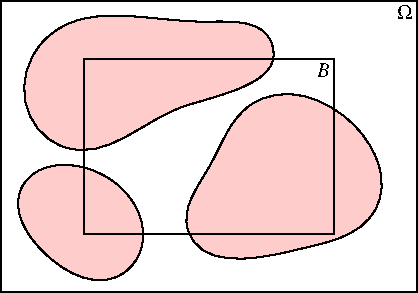
\includegraphics{images/algebra-1}
\end{center}
\caption{Ereignisalgebra mit ausgezeichneten Ereignis $B$\label{bedingt1}}
\end{figure}
\begin{figure}
\begin{center}
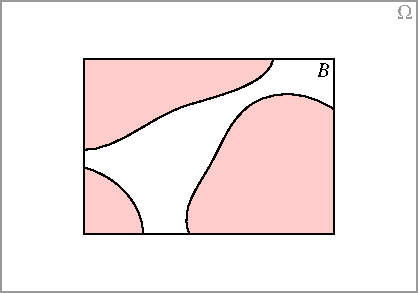
\includegraphics{images/algebra-2}
\end{center}
\caption{Ereignisalgebra wie in Abbildung \ref{bedingt1} eingeschränkt auf das Ereignis $B$\label{bedingt2}}
\end{figure}
In der Praxis fragt man oft nach der Verkettung von Umständen: hat ein
Patient bessere Heilungschancen wenn er dieses neue Medikament nimmt?
Man könnte das auch so formulieren: ist das Ereignis
``Patient wird gesund, unter der Voraussetzung, dass er das Medikament nimmt''
wahrscheinlicher als das Ereignis ``Patient wird gesund''? Wir müssen
also aus der Ereignis\-algebra der Patienten eine neue bilden, die nur
aus den Patienten besteht, welche das Medikament genommen haben.

Wenn $(\Omega, {\cal A})$ eine Ereignisalgebra ist, und 
$B\in{\cal A}$ ein Ereignis (Abbildung~\ref{bedingt1}),
dann kann man eine neue Ereignisalgebra
$(\Omega_{|B}, {\cal A}_{|B})$ wie folgt bilden (Abbildung~\ref{bedingt2}).
Die Menge der Elementarereignisse ist
\[
\Omega_{|B}=B
\]
und die Menge der Ereignisse
\[
{\cal A}_{|B}=\{A\cap B\;|\; A\in{\cal A}\}.
\]
Es wäre noch nachzuprüfen, dass diese Menge alle Axiome einer
Ereignisalgebra erfüllt sind\footnote{Da diese technischen Feinheiten 
für die Zwecke dieses Skripts von untergeordneter Bedeutung sind, verzichten
wir auf die explizite Verifikation.}.
Diese Konstruktion macht $B$ zum sicheren Ereignis, d.~h.~in der ``Welt''
$(\Omega_{|B},{\cal A}_{|B})$ trifft $B$ immer ein (Abbildung~\ref{bedingt2}).
In $(\Omega_{|B},{\cal A}_{|B})$ muss man also davon ausgehen, dass $B$
bereits eingetroffen ist.
Man liest $\Omega_{|B}$ auch als ``$\Omega$ bedingt $B$''.

Wenn nun auf $(\Omega, {\cal A})$ eine Wahrscheinlichkeitsfunktion $P$
gegeben ist, kann man auch $P_{|B}$ bilden, indem man setzt
\begin{equation*}
P_{|B}(A)=\frac{P(A\cap B)}{P(B)},
\end{equation*}
der Nenner $P(B)$ stellt dabei sicher, dass $P_{|B}(\Omega_{|B})=P_{|B}(B)=1$.

\begin{definition}
\label{def-bedingte-wahrscheinlichkeit}
Die bedingte Wahrscheinlichkeit eines Ereignisses $A$ unter der Bedingung
$B$ ist
\[
P(A|B)=\frac{P(A\cap B)}{P(B)}.
\]
Man liest dies auch als ``Wahrscheinlichkeit von $A$ bedingt $B$''.
\end{definition}

Auch hier wäre nachzuprüfen, dass die Rechenregeln für eine
Wahrscheinlichkeitsfunktion erfüllt sind.
Um also die Wahrscheinlichkeit in dieser Welt zu berechnen,
in der $B$ bereits eingetroffen ist, 
muss man $P(A\cap B)$ berechnen können.
Dies sollte Motivation genug sein, Rechenregeln für
$P(A\cap B)$ aufzustellen, die uns bisher fehlen.

\subsection{Wahrscheinlichkeit von \texorpdfstring{$A\cap B$}{A geschnitten B}}
\begin{figure}
\begin{center}
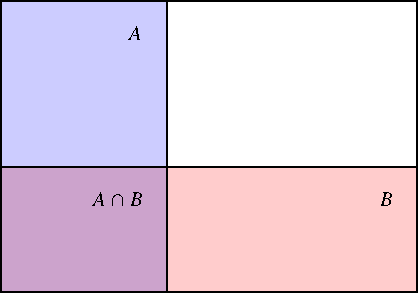
\includegraphics{images/abhaengigkeit-1}
\end{center}
\caption{Unabhängige Ereignisse.
Die Ereignisse sind so dargestellt,
dass ihre Wahrscheinlichkeit proportional zur Fläche ist.
$P(A)$ und $P(B)$
entsprechen dem Teilverhältnis, in dem $A$ bzw.~$B$ die Seite des grossen
Rechtecks teilen.
$P(A\cap B)=P(A)\cdot P(B)$\label{unabhaengig}}
\end{figure}
\begin{figure}
\begin{center}
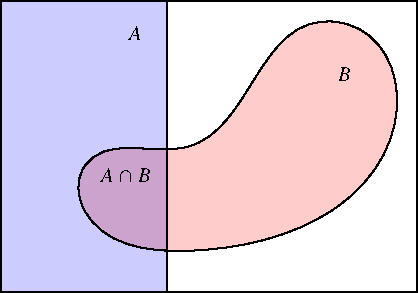
\includegraphics{images/abhaengigkeit-2}
\end{center}
\caption{Abhängige Ereignisse.
$P(A\cap B)$ ist offensichtlich viel kleiner
als $P(A)\cdot P(B)$.
$A$ wird unwahrscheinlicher, wenn bereits $B$ eingetreten
ist.
\label{abhaengig}}
\end{figure}
Der Grund dafür, dass es keine einfache Rechenregel für die Berechnung von 
$P(A\cap B)$ aus $P(A)$ und $P(B)$ gibt, wird mit der
Visualisierung der Ereignisse im in einem Venn-Diagramm sofort klar.
Die Elementarereignisse seien so angeordnet, dass $A$ das durch eine
vertikale Strecke abgetrennte, linke Teilrechteck von $\Omega$ ist.
Ausserdem
sollen Sie so angeordnet sein, dass die Wahrscheinlichkeit dem
Flächeninhalt im Diagramm entspricht.

Das Ereignis $B$ ist jetzt im Allgemeinen eine Teilmenge, die sowohl $A$ 
als auch $\bar A$ schneidet.
Die Wahrscheinlichkeit $P(A \cap B)$ entspricht
der Fläche der Schnittmenge im Diagramm.
Im Allgemeinen haben wir
nur aus $P(B)$ nicht genügend Information um zu entscheiden, welche
``Form'' $A\cap B$ hat, wir können also nicht erwarten, dass wir $P(A\cap B)$
berechnen können.

Wenn sich $B$ ebenfalls mittels einer horizontalen Strecke als Rechteck
einzeichnen lässt, dann ist $P(B)$ auch das Teilverhältnis, in dem
die Strecke die vertikale Kante des Diagramms teilt.
Somit kann man $P(A\cap B)$
als Flächeninhalt des Schnittrechtecks berechnen: $P(A\cap B)=P(A)\cdot P(B)$.
Die Voraussetzung bedeutet, dass das Eintreffen von $B$ nicht wahrscheinlicher
oder weniger
wahrscheinlich wird, wenn $A$ eintrifft.
Das Eintreffen von $B$ hängt also
nicht mit dem Eintreffen von $A$ zusammen.

\begin{definition}
\label{def-unabhaengige-ereignisse}
Die Ereignisse $A$ und $B$ heissen {\em unabhängig}, wenn gilt:
\[
P(A\cap B) = P(A)\cdot P(B).
\]
\end{definition}

Beim Würfeln sagt die Erfahrung, dass sich ein Würfel nicht an den
letzten Wurf erinnern kann, d.~h.~der Ausgang des letzten Wurfes hat
keinen Einfluss auf den nächsten Wurf.
Die Ereignisse ``im ersten
Wurf wird eine 5 gewürfelt'' und ``im zweiten Wurf wird eine 6 gewürfelt''
sind also unabhängig.
Die Wahrscheinlichkeit, dass mit einem Würfel
erst eine 5, dann eine 6 gewürfelt wird, ist also
\begin{align*}
P(A\cap B)&=P(\text{``erster Wurf: 5''}\cap\text{``zweiter Wurf: 6''})\\
&=P(\text{``erster Wurf: 5''})\cdot P(\text{``zweiter Wurf: 6''})\\
&=\frac1{36}.
\end{align*}

\subsection{Bedingte Wahrscheinlichkeit}
Im vorangegangenen Abschnitt wurde bereits die bedingte Wahrscheinlichkeit
$P_{|B}(A)$ konstruiert, die wir auch
\[
P(A|B)=\frac{P(A\cap B)}{P(B)}
\]
schreiben.
Die Bedeutung des Symbols $P(A|B)$ ist die folgende.
Bei der
Bestimmung der Wahrscheinlichkeit werden nur diejenigen Experimente
berücksichtigt, bei denen das Ereignis $B$ eingetreten ist.
Alle anderen Experimente interessieren nicht.

\subsubsection{Beispiel: Autounfälle und Alkohol}
Wenn jemand sagt, 50\%
der tödlichen Autounfälle geschehen unter Alkoholeinfluss, dann
meint er genau genommen eigentlich folgendes.
Wir machen ein Experiment,
bei dem wir jeden Autounfall untersuchen.
Das Ereignis $T$ umfasst alle
tödlich ausgehenden Autounfälle, das Ereignis $A$ all jene, bei denen
Alkohol im Spiel war.
Uns interessieren jetzt nur noch die tödlichen
Unfälle, also die, bei denen das Ereignis $T$ eingetreten ist. 
Die anderen untersuchen wir gar nicht mehr.
Jetzt möchten wir die
Wahrscheinlichkeit wissen, dass Alkohol im Spiel war, aber nur noch
bei den tödlichen Unfällen.
Dies ist $P(A|T)$, also gilt
$P(A|T)=50\% = 0.5$.
$P(T|A)$ ist hingegen ganz etwas anderes.
Hier fragt man danach,
wie wahrscheinlich es ist, dass bei einem Autounfall unter Alkoholeinfluss
ein Toter zu beklagen ist.

\subsubsection{Beispiel: Rauchen und Lungenkrebs}
\index{Rauchen}
\index{Lungenkrebs}
In einem Zeitungsartikel gefunden: Die Wahrscheinlichkeit, dass ein Raucher
Lungenkrebs entwickelt, ist 15\%, bei einem Nichtraucher ist sie nur 1\%.
Das Experiment besteht darin, einen Menschen zu beobachten.
Einige
davon sind Raucher (Ereignis $R$), einige entwickeln Lungenkrebs (Ereignis $L$).
Betrachtet man nur die Raucher, so ist die Wahrscheinlichkeit für
Lungenkrebs 15\%, also
\[
P(L|R)=0.15
\]
Betrachtet man nur die Nichtraucher, also das Ereignis $\bar R$, findet
man 
\[
P(L|\bar R)=0.01.
\]
Der Artikel liefert aber keine Auskunft darüber, wie viele der
Lungenkrebskranken auch Raucher sind, denn das wäre die Wahrscheinlichkeit
$P(R|L)$.

\subsubsection{Zusammenhang zwischen \texorpdfstring{$P(A\cap B)$}{P(A geschnitten B)}, \texorpdfstring{$P(A|B)$}{P(A bedingt B)} und \texorpdfstring{$P(B|A)$}{P(B bedingt A)}}
In allen drei Fällen geht es um die Wahrscheinlichkeit des Eintretens
von $A$ und von $B$, allerdings jeweils in verschiedenem
Zusammenhang.
\begin{center}
\begin{tabular}{|c|l|c|}
\hline
Wahrscheinlichkeit&Übersetzung&Scope\\
\hline
$P(A\cap B)$&\strut Wahrscheinlichkeit, dass $A$ und $B$ eintreten\strut &$\Omega$\\
%\hline
$P(A|B)$&\begin{minipage}[t]{3.0in}\strut Wahrscheinlichkeit, dass $A$ eintritt, wenn $B$ schon eingetreten ist\strut \end{minipage}&$B$\\
%\hline
$P(B|A)$&\begin{minipage}[t]{3.0in}\strut Wahrscheinlichkeit, dass $B$ eintritt, wenn $A$ schon eingetreten ist\strut \end{minipage}&$A$\\
\hline
\end{tabular}
\end{center}
(Vergleiche auch Abbildung~\ref{condprob}.)
\begin{figure}
\begin{center}
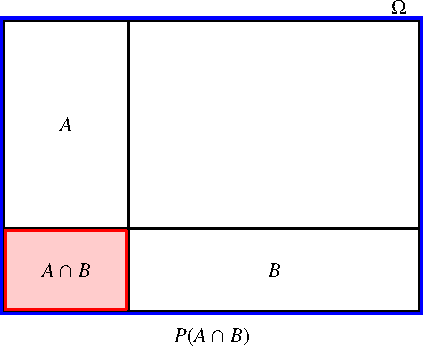
\includegraphics[width=0.3\hsize]{images/abhaengigkeit-3}\quad
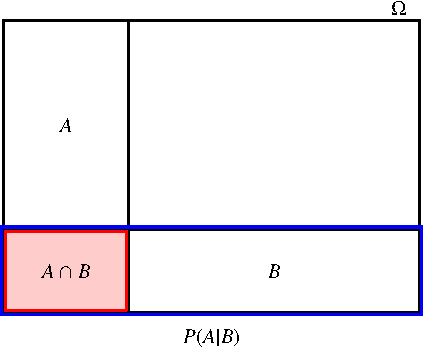
\includegraphics[width=0.3\hsize]{images/abhaengigkeit-5}\quad
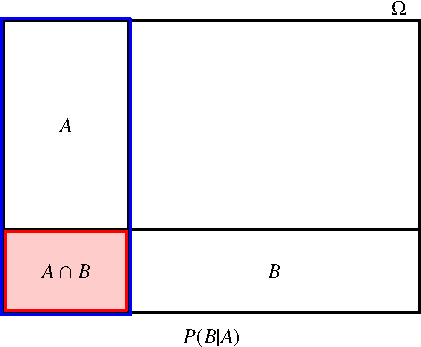
\includegraphics[width=0.3\hsize]{images/abhaengigkeit-4}
\end{center}
\caption{Wahrscheinlichkeit von $A\cap B$ in jeweils anderer Umgebung
\label{condprob}}
\end{figure}

\subsection{Zerlegung eines Wahrscheinlichkeitsraumes}
Der
Begriff der bedingten Wahrscheinlichkeit ermöglicht,
ein Wahrscheinlichkeitsproblem in möglicherweise einfachere, jedenfalls
kleinere Probleme zu zerlegen.
Wenn bei einem Experiment zwei Zustände
eintreten, die sich gegenseitig ausschliessen, können wir die 
Wahrscheinlichkeit bestimmen, unter denen die weiteren Resultate
des Experiments eintreten, jedoch unter der Vorbedingung, dass einer
der benannten Zustände bereits eingetreten ist.
Wenn wir nun auch
noch die Wahrscheinlichkeit jedes Zustandes kennen, müsste es doch
möglich sein, auch die Wahrscheinlichkeit der weiteren Resultate zu
ermitteln.
% TODO Missing Example
Im obigen Beispiel der Meinungsumfrage ist anschaulich klar, dass man die
Wahrscheinlichkeit für ``Ja'' berechnen kann, wenn man einerseits die
Wahrscheinlichkeit für ``Ja'' in  jeder Altersklasse kennt, und andererseits
weiss, wie die Altersklassen in der Bevölkerung verteilt sind.

\begin{figure}
\begin{center}
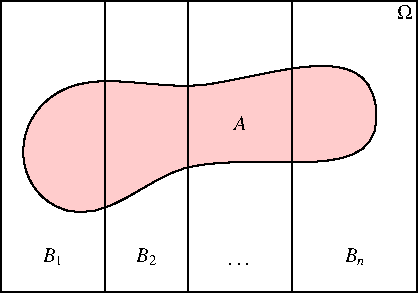
\includegraphics{images/total-1.pdf}
\end{center}
\caption{Wahrscheinlichkeitsraum $\Omega$, der sich in die in die
Ereignisse $B_1,B_2,\dots,B_n$ zerlegen lässt.\label{zerlegung}}
\end{figure}
Wir versuchen, das etwas formaler zu schreiben
(siehe Abbildung \ref{zerlegung}):
Sind $B_i$ mit $1\le i$ paarweise
disjunkte Ereignisse
in einer Ereignisalgebra $(\Omega,{\cal A})$, für welche ausserdem
gilt
\[
\bigcup_{i=0}^{n}B_i = \Omega,
\]
dann kann man die Wahrscheinlichkeit von $A$ aus den bedingten
Wahrscheinlichkeiten der Teile $A\cap B_i$ und $B_i$ wieder zusammensetzen.
Bekannt sind die Wahrscheinlichkeiten
$P(B_i)$, die Wahrscheinlichkeit der Zustände, und
$P(A|B_i)$, die Wahrscheinlichkeit, dass $A$ eintritt, unter der Bedingung
das $B_i$ bereits eingetreten ist.
Nach Definition ist $P(A|B_i)=P(A\cap B_i)/P(B_i)$, also
$P(A|B_i)\cdot P(B_i) = P(A\cap B_i)$.
Die Vereinigung der Ereignisse $A\cap B_i$ ist
\[
\bigcup_{i=0}^{n} A\cap B_i=A\cap\bigcup_{i=0}^{n}B_i=A,
\]
und die Mengen $A\cap B_i$ sind disjunkt.
Also kann man die Summe ihrer
Wahrscheinlichkeiten mit der Additionsformel ausrechnen:
\[
\sum_{i=0}^{n}P(A\cap B_i)=P\biggl(\bigcup_{i=0}^{n}A\cap B_i\biggr)=P(A).
\]
Andererseits
haben wir oben bereits $P(A\cap B_i)$ bestimmt, wir können
also einsetzen und erhalten:
\[
P(A)=\sum_{i=0}^{n}P(A|B_i)\cdot P(B_i).
\]
Somit lässt sich tatsächlich die Wahrscheinlichkeit eines Ereignisses
aus den bedingten Wahrscheinlichkeiten und den Wahrscheinlichkeiten
der Bedingungen errechnen.
Wir fassen diese Erkenntnis in folgendem Satz zusammen.
\index{Wahrscheinlichkeit!totale}
\begin{satz}
Ist $B_i$ eine Folge paarweise disjunkter Mengen mit $\bigcup_{i=0}^{n}B_i=\Omega$, dann gilt für jedes Ereignis $A$
\[
P(A)=\sum_{i=0}^{n}P(A|B_i)\cdot P(B_i).
\]
\end{satz}
Dieser Satz heisst auch der {\em Satz von der totalen Wahrscheinlichkeit},
da er die Wahrscheinlichkeit eines Ereignisses aus den bedingten
Wahrscheinlichkeiten unter verschiedenen Voraussetzungen und der
Wahrscheinlichkeit des Eintretens dieser Voraussetzungen rekonstruiert.
Dieser Satz ist die ``wahrscheinlichkeitstheoretisch Form einer
Fallunterscheidung'': man kennt die Fälle $B_i$, und deren Wahrscheinlichkeit
$P(B_i)$, sowie die Wahrscheinlichkeit $P(A|B_i)$, dass $A$ im Falle 
$B_i$ eintritt.
Die Formel über die totale Wahrscheinlichkeit
liefert daraus wieder $P(A)$.

Wir bemerken noch, dass es gar nicht unbedingt nötig ist, dass die Mengen
$B_i$ ganz $\Omega$ ausschöpfen, es würde auch
genügen, wenn die Wahrscheinlichkeit $0$ ist, dass $A$ eintritt
unter der Bedingung,
dass bereits $\bigcup_{i=0}^{n}B_i$ eingetreten ist.
Für den
Experimentator bedeutet das, dass er nur jene Vorbedingungen $B_i$
berücksichtigen muss, unter denen sein Experiment ``funktioniert'',
alle anderen möglichen Zustände haben keinen Einfluss auf
die Wahrscheinlichkeit seiner Resultate.
Man darf beim Experimentieren also durchaus einzelne Resultate
verwerfen, wenn man weiss, was man tut!

\subsubsection{Studienerfolg}
Die folgenden Zahlen sind erfunden, und dienen nur der Illustration
des Prinzips.
Eine Statistik hat die Wahrscheinlichkeit für den
Studienerfolg untersucht, und folgende Resultate erhalten.
Die Studierenden setzen sich zusammen aus 60\% BMS, 30\% Kantonsschüler
und Übertritte von anderen Hochschulen.
Die Wahrscheinlichkeit
das Studium erfolgreich abzuschliessen, ist für BMS 80\%,
für Kantonsschüler 90\%, 85\% für die Übertreter von anderen
Hochschule.
Wie gross ist die Wahrscheinlichkeit für den Studienerfolg?

$\Omega$ ist die Menge aller Studienversuche.
60\% davon bilden das
Ereignis $B$ bestehend aus Studienversuchen, die im Anschluss an die BMS
erfolgen.
30\% machen das Ereignis $K$ mit den Kanti-Abgängern aus,
10\% das Ereignis $A$ mit Übertritten von anderen Hochschulen.
Es ist klar, dass 
\[
\Omega = B \cup K\cup A.
\]
Gefragt ist die Wahrscheinlichkeit des Ereignisses $E$, welches
die erfolgreich abgeschlossenen Studienversuche beinhaltet.
Für die Wahrscheinlichkeit gilt nach dem Satz über die totale
Wahrscheinlichkeit
\begin{align*}
P(E)&=P(E|B)P(B)+P(E|K)P(K)+P(E|A)P(A).
\\
    &= 80\%\cdot 60\%
     + 90\%\cdot 30\%
     + 85\%\cdot 10\%
\\
&=0.8\cdot 0.6 + 0.9 \cdot 0.3 + 0.85 \cdot 0.1 = 0.835.
\end{align*}

\subsubsection{Würfelspiel}
Wir betrachten nochmals das Beispiel Würfeln mit zwei Würfeln, wobei
bei einem Pasch im ersten Wurf noch genau einmal gewürfelt wird.
Wir möchten die Wahrscheinlichkeit berechnen, dass die totale Augensumme
mindestens 10 ist.
Wir nennen dieses Ereignis $Z$.

Zunächst kann man unterteilen für den Fall, dass im ersten Wurf
ein Pasch (Ereignis $P$) geworfen wird.

Es gilt nach dem Satz über die totale Wahrscheinlichkeit
\[
P(Z) = P(Z|P) P(P) + P(Z|\bar P) P(\bar P).
\]
Selbstverständlich ist $P(\bar P)=1-P(P)$, so dass man $P(Z)$ bereits
vereinfachen kann:
\[
P(Z) = P(Z|P) P(P) + P(Z|\bar P) (1-P(P)).
\]
Man kann aber das Ereignis $P$ noch weiter unterteilen in die
Ereignisse $P_k$, mit $1\le k\le 6$, also
\begin{align*}
P(P)&=
P(P_1)+
P(P_2)+
P(P_3)+
P(P_4)+
P(P_5)+
P(P_6),
\\
P(Z|P)
&=
P(Z|P_1)P(P_1|P)+
P(Z|P_2)P(P_2|P)+
P(Z|P_3)P(P_3|P)
\\
&\qquad +
P(Z|P_4)P(P_4|P)+
P(Z|P_5)P(P_5|P)+
P(Z|P_6)P(P_6|P).
\end{align*}
Die Ereignisse haben wir auch früher schon untersucht, daraus kann
man einige Wahrscheinlichkeiten bereits ablesen:
\begin{align*}
P(Z|P_6)&=1,\\
P(Z|P_5)&=1,\\
P(Z|P_4)&=1,
\end{align*}
denn in allen diesen Fällen erreicht man mit dem zweiten Wurf mit
Sicherheit zehn oder mehr.

\subsection{Ziegen und Autos} \label{ziegen:autos}
Marylin vos Savant hat in einer Kolumne ein Gedankenexperiment vorgestellt.
In einer Quiz-Show muss der Kandidat eine von drei Türen wählen, wobei
sich hinter einer der Türen ein Auto versteckt, hinter den anderen Zweien
ein Ziege.
Das Ziel des Spiels ist, das Auto zu gewinnen.
Nach der Wahl
durch den Kandidaten öffnet der Quizmaster eine der Türen, hinter der sich
eine Ziege befindet, nicht aber die Tür, die der Kandidat gewählt hat.
Der Kandidat hat jetzt nochmals die Möglichkeit, die Tür zu wechseln.
Welche Strategie soll er wählen.
Bei der ersten Auswahl bleiben, oder
wechseln?

Um die Frage zu beantworten berechnen wir die Gewinnwahrscheinlichkeit
für jede der Strategien.
Zunächst die ``Bleibe''-Strategie.
Es ist die
Wahrscheinlichkeit für einen Gewinn $P(G)$ auszurechnen.
Hinter der zunächst
gewählten Tür kann sich ein Auto (Ereignis $A$) befinden, oder eine Ziege
(Ereignis $Z$).
Es ist natürlich $A\cap Z=\emptyset$ und $A\cup Z=\Omega$.
Also gilt
\begin{equation}
P(G)=P(G|A) P(A) + P(G|Z)P(Z).
\label{ziegenformel}
\end{equation}
Natürlich ist $P(A)=\frac13$ und $P(Z)=\frac23$.
$P(G|A)$ ist die Wahrscheinlichkeit mit der ``Bleibe''-Strategie zu
gewinnen, wenn hinter der zunächst gewählten Tür ein Auto war: diese
ist natürlich $1$.
Ebenso verliert man mit Sicherheit, wenn hinter der
Tür eine Ziege war: $P(G|Z)=0$, also
\[
P(G)=P(G|A)P(A)+P(G|Z)P(Z)=1\cdot \frac13 + 0\cdot\frac 23=\frac13.
\]

Für die ``Wechsel''-Strategie gilt natürlich auch die Formel
\ref{ziegenformel}, aber die bedingten Wahrscheinlichkeiten sind verschieden.
Wenn man ein Auto gewählt hatte, und wechselt, verliert man, also $P(G|A)=0$.
Hat man ein Ziege erwischt, und wechselt, bekommt man das Auto, denn die
zweite Ziege kann man ja nicht erwischen, deren Tür hat der Quiz-Master
geöffnet.
Also ist $P(G|Z)=1$.
Somit folgt jetzt
\[
P(G)=P(G|A)P(A)+P(G|Z)P(Z)=0\cdot\frac13+1\cdot\frac23=\frac23.
\]
Mit der Wechselstrategie ist also die Wahrscheinlichkeit, zu gewinnen,
doppelt so gross, wechseln lohnt sich also auf jeden Fall.


\subsection{Wahrscheinlichkeitsvektoren und -matrizen}
Der Satz von der totalen Wahrscheinlichkeit kann auch in Matrixform
geschrieben werden:
\begin{align*}
P(A)&=P(A|B_1)P(B_1)+\dots+P(A|B_n)P(B_n)
=
\begin{pmatrix}
P(A|B_1)&\dots&P(A|B_2)
\end{pmatrix}
\begin{pmatrix}
P(B_1)\\\vdots\\P(B_n)
\end{pmatrix}
\end{align*}
Der Spaltenvektor
\[
\begin{pmatrix}
P(B_1)\\\vdots\\P(B_n)
\end{pmatrix}
\]
hat die Eigenschaften, dass alle seine Einträge zwischen $0$ und $1$
liegen, und ihre Summe $1$ gibt.
\index{Wahrscheinlichkeitsvektor}
Ein solcher Vektor heisst {\it Wahrscheinlichkeitsvektor}.

Die Matrizenschreibweise erlaubt, auch die totalen Wahrscheinlichkeiten
für mehrere Ereignisse $A_1,\dots,A_m$ gleichzeitig zu berechnen:
\[
\begin{pmatrix}
P(A_1)\\
P(A_2)\\
\vdots\\
P(A_m)
\end{pmatrix}
=
\begin{pmatrix}
P(A_1|B_1) & P(A_1|B_2) & \dots &P(A_1|B_n)\\
P(A_2|B_1) & P(A_2|B_2) & \dots &P(A_2|B_n)\\
\vdots     & \vdots     & \ddots&\vdots\\
P(A_m|B_1) & P(A_m|B_2) & \dots &P(A_m|B_n)\\
\end{pmatrix}
\begin{pmatrix}
P(B_1)\\
P(B_2)\\
\vdots\\
P(B_n)
\end{pmatrix}.
\]
Sind die Ereignisse $A_i$ ebenfalls paarweise disjunkt und decken ganz
$\Omega$ ab, dann sind auch die Spalten von der Matrix $(P(A_i|B_j))$
jeweils Wahrscheinlichkeitsvektoren.
\index{Wahrscheinlichkeitsmatrix}
Eine solche Matrix heisst {\it Wahrscheinlichkeitsmatrix}.

\subsection{Satz von Bayes} \label{satz-von-bayes}
\index{Bayes, Satz von}
Für zwei beliebige Ereignisse mit $A$ und $B$ mit nicht verschwindender
Wahrscheinlichkeit gilt
\[
P(A|B)\cdot P(B)= P(A\cap B)=P(B|A)\cdot P(A),
\]
und es folgt
\[
P(A|B)=\frac{P(B|A)\cdot P(A)}{P(B)}.
\]
Dieser Zusammenhang ist bekannt als der Satz von Bayes:
\begin{satz}[Satz von Bayes]
Für zwei Ereignisse $A$ und $B$ mit $P(B)\ne0$ gilt
\[
P(A|B)=\frac{P(B|A)\cdot P(A)}{P(B)}.
\]
\end{satz}
Die Bedeutung dieses Satzes besteht darin, dass er die Schlussrichtung
umzukehren erlaubt.
Die bedingte Wahrscheinlichkeit $P(A|B)$ ist ja die
Wahrscheinlichkeit, dass ein das Ereignis $A$ eintritt, wenn $B$ bereits
eingetreten ist.
Sie erlaubt, eine Wette einzugehen, dass $A$ eintreten
wird, wenn $B$ bereits eingetreten ist.
Der Satz von Bayes ermöglicht
also, auch eine Wette für $B$ einzugehen, wenn $A$ bereits eingetreten
ist.
Im Gegensatz zur Schlussweise in der Logik, die niemals umkehrbar ist,
kann man auf Wahrscheinlichkeiten basierende Schlüsse umkehren.

\subsubsection{Was bedeutet ein positiver HIV-Test?}
\begin{figure}
\begin{center}
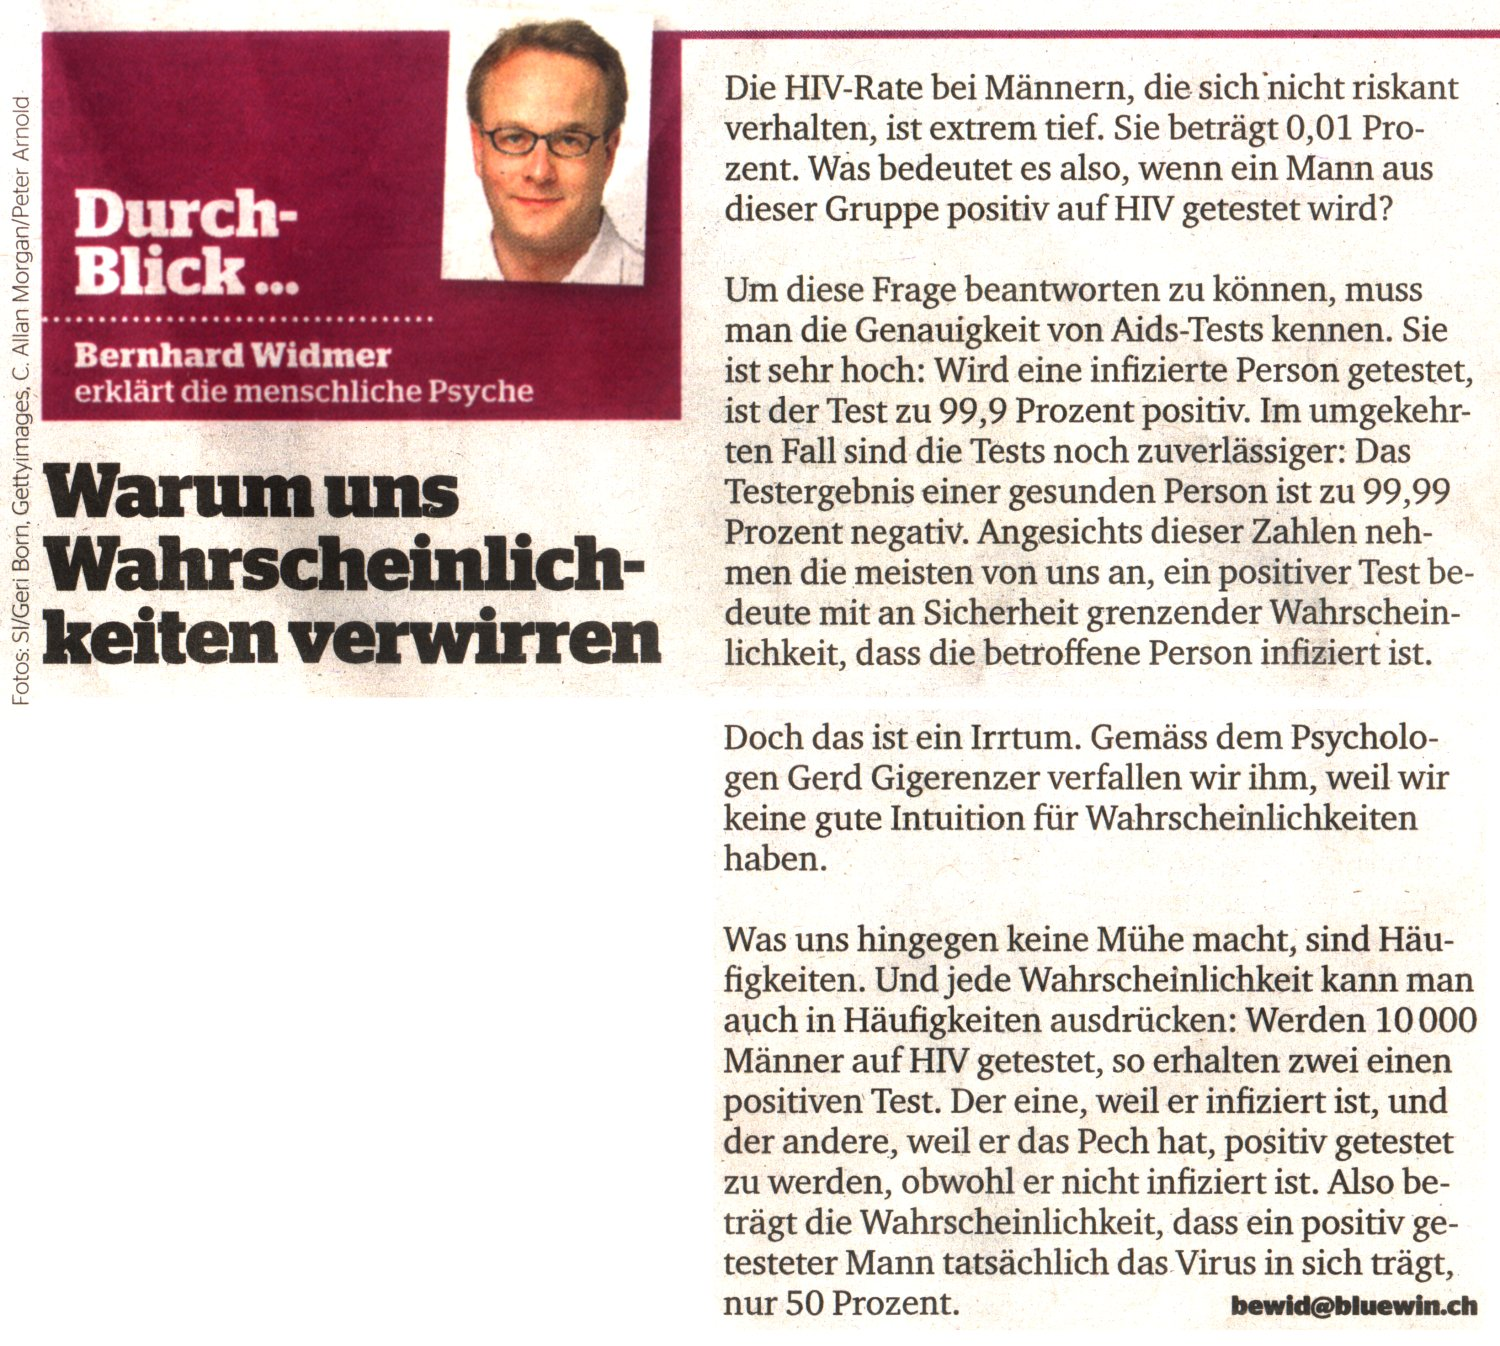
\includegraphics[width=\hsize]{graphics/aids-300}
\end{center}
\caption{``Blick am Abend'' vom 12.~August 2008\label{aids}}
\end{figure}
Im ``Blick am Abend'' vom 12.~August 2008 erschien der Artikel in Abbildung 
\ref{aids} mit dem Titel ``Warum uns Wahrscheinlichkeiten verwirren''.
Darin ist von folgenden Ereignissen die Rede, die sich auf sich nicht riskant
verhaltende Männer ($=\Omega$) beziehen.
\index{HIV-Test}
\begin{enumerate}
\item Ereignis $H$: Ein Mann ist HIV-infiziert.
\item Ereignis $T$: ein HIV-Test ergibt ein positives Resultat.
\end{enumerate}
Der Artikel teilt uns zudem ein paar Wahrscheinlichkeiten mit:
\begin{itemize}
\item HIV-Rate bei Männern, die sich nicht riskant verhalten:
$P(H)=0.0001$.
\item Wahrscheinlichkeit, dass bei einer infizierten Person der Test
ein positives Resultat ergibt: $P(T|H)=0.999$.
\item Wahrscheinlichkeit, dass bei einer gesunden Person der Test negativ
ist: $P(\bar T|\bar H)=0.9999$.
\end{itemize}
Wie gross ist die Wahrscheinlichkeit, dass ein sich nicht riskant verhaltender
Mann tatsächlich HIV hat, wenn er einen positiven HIV-Test hat? Wie
gross ist $P(H|T)$?

Der Satz von Bayes liefert die Antwort:
\begin{equation}
P(H|T)=\frac{P(T|H)\cdot P(H)}{P(T)}
\label{aidsprobability}
\end{equation}
Darin sind fast alle Grössen direkt aus dem Artikel ablesbar, nur $P(T)$ muss
noch bestimmt werden.
Dazu dient der Satz über die totale Wahrscheinlichkeit,
den wir auf die Tatsache anwenden, dass ein sich nicht riskant verhaltender
Mann entweder HIV hat oder nicht: $\Omega=H\cup \bar H$.
\begin{align*}
P(T)
&=P(T|H)\cdot P(H)+P(T|\bar H)\cdot P(\bar H)\\
&=P(T|H)\cdot P(H)+(1-P(\bar T|\bar H))\cdot (1 - P(H))\\
&=0.999\cdot 0.0001+(1-0.9999)\cdot(1-0.0001)\\
&=0.00019989\simeq 0.0002
\end{align*}
Eingesetzt in (\ref{aidsprobability}) ergibt sich jetzt das Resultat
\[
P(H|T)=\frac{0.999\cdot 0.0001}{0.0002}=.4995\simeq 0.5
\]
oder mit anderen Worten, auch wenn der HIV-Test positiv ist, ist
die Wahrscheinlichkeit für einen sich nicht riskant verhaltenden Mann,
tatsächlich HIV-infiziert zu sein, nur $50\%$.

